
\section{Markov Decision Process}
Ein Markov Decision Process (MDP) modelliert die Interaktion eines Agenten mit seiner Umgebung
\cite{sutton1998rlintro}. Der Agent kann hierfür zu jedem diskreten Zeitpunkt $t$ eine
Aktion $a_t$ anhand des für ihn sichtbaren Systemzustands $o_{t}$ auswählen und durchführen,
wodurch das System vom Zustand $s_t$ in den Zustand $s_{t+1}$ überführt wird.
Als Rückmeldung erhält der Agent eine Belohnung $r_t$ und eine aktualisierte
Sicht $o_{t+1}$ auf den neuen Systemzustand $s_{t+1}$.\\

\begin{figure}[h]
  \centering
  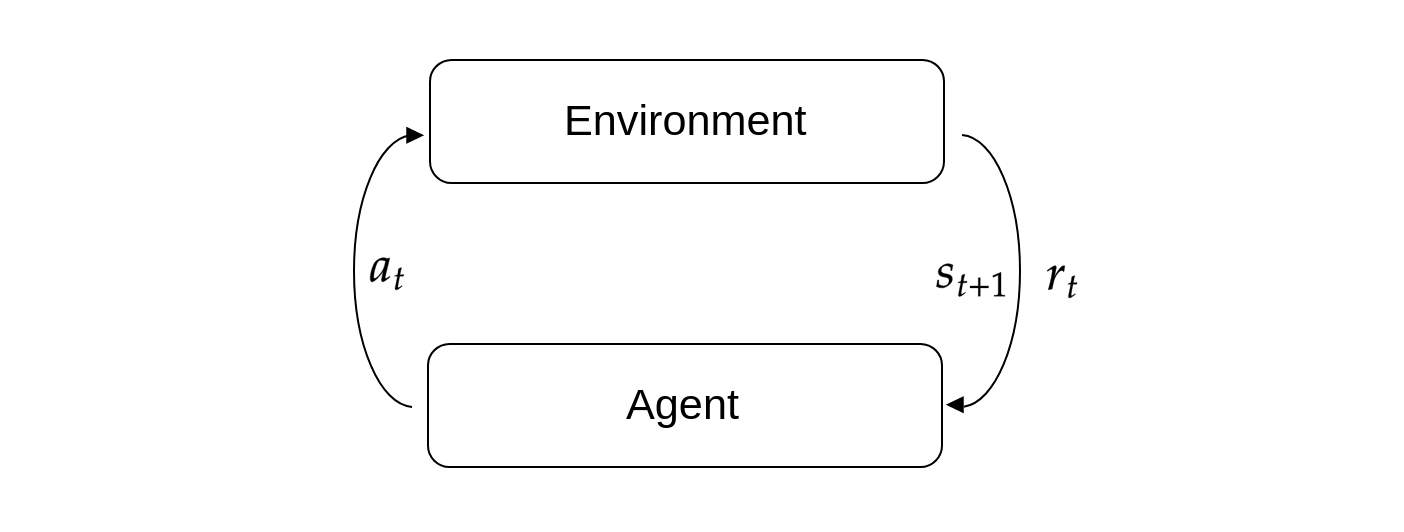
\includegraphics[width = 0.65\textwidth]{imgs/markov_decision_process}
  \caption{Veranschaulichung eines Markov Decision Process}
  \label{fig:MDP}
\end{figure}

Um einen MDP zu modellieren, muss die Umgebung eine Übergangsfunktion
$\rho: S \times A \mapsto S \times R$ bereitstellen, welche den Ausgangszustand $s_t$
nach Durchführung der Aktion $a_t$ auf den resultierenden Zustand $s_{t+1}$
und die erhaltene Belohnung $r_t$ abbildet; $S$, $A$ und $R$ beschreiben jeweils
den Zustands-, Aktions- und Belohnungsraum.
In den meisten realitätsnahen Anwendungsfällen ist zudem die Wahrnehmung eines Agenten
bezüglich seiner Umgebung unvollständig, sodass der Agent nur einen Ausschnitt
des Gesamtsystems sieht, beispielsweise durch entsprechende Sensoren. Es wird folglich
von einem Partially Observable Markov Decision Process (POMDP) gesprochen,
da der Agent nur den für ihn sichtbaren Teil $o_t$ des gesamten Systemzustandes
$s_t$ wahrnimmt. Eine zusätzliche Abbildung $\omega: S \mapsto O$ übersetzt den
Systemzustand $s_t$ in den für den Agenten sichtbaren Teilzustand $o_t$ des
Wahrnehmungsraums $O$ (engl. Observation Space).\\

Durch die abstrakte Definition der Übergangsfunktion sind vielseitige Umsetzungen
einer Umgebung möglich, unter anderem realitätsgetreue Simulationen mit physikalischen
Formeln, zufallsbasierte Modelle oder gar trainierte Neuronale Netze.
Ein POMDP liegt auch insbesondere beim Autonomen Fahren vor, da der Fahragent mittels
Sensorik immer nur einen Ausschnitt der Realität wahrnimmt. Beispielsweise kann
ein Objekt durch ein anderes Objekt temporär verdeckt sein, sodass es der Agent
nicht sehen kann. Dennoch muss der Agent auch latente Wahrnehmungen in seine
Entscheidungen mit einbeziehen.\\

Die durch die Übergangsfunktion $\rho$ definierten Transitionen zwischen den Zuständen
spannen einen Spielegraph auf, bei dem die Zustände den Knoten und die im jeweiligen
Zustand wählbaren Aktionen den gerichteten Kanten entsprechen. Durch die Interaktion
des Agenten mit seiner Umgebung wird der Graph durchlaufen, was sich in einer
Abfolge an Zuständen, Aktionen und Belohnungen in Form einer Trajektorie $\tau$
manifestiert. Eine Trajektorie kann als eine Menge an Erfahrungen
$(s_t, a_t, r_t, s_{t+1})$, den sogenannten SARS-Tupeln, für die jeweiligen
Zeitschritte $t \in \{ t_0 ... t_{term} \}$ verstanden werden.
Sobald ein Terminalzustand des Spielegraphs erreicht wird, endet die Trajektorie.
Der Zeitabschnitt zwischen dem initialen Zeitpunkt $t_0$ und dem terminalen Zeitpunkt
$t_{term}$ wird im Kontext des Bestärkenden Lernens auch als Episode bezeichnet.

\begin{equation}
\begin{aligned}
\tau = \{ (s_{t}, a_{t}, r_t, s_{t+1}) | t \in \{ t_0 ... t_{term} \}
\land \rho(s_t, a_t) = (s_{t+1}, r_t) \}
\end{aligned}
\end{equation}

Zur Lösung eines MDP verfolgt der Agent das Ziel, die über eine Episode gesammelten
Belohnungen (engl. Return, Gain) zu maximieren, was mit der Formel
$G_t = \sum_{l=0}^{\infty} r_{t+l} \cdot \gamma^l$ ausgedrückt werden kann.
$\gamma \in (0, 1)$ stellt einen Diskontierungsfaktor dar, der Belohnungen in
der Gegenwart stärker als Belohnungen in der Zukunft gewichtet, sodass weit in der
Zukunft liegende Belohnungen kaum noch zum Return beitragen, da
$\lim \limits_{l \to \infty} r_{t+l} \cdot \gamma^l = 0$.
Für Spielegraphen ohne Terminalzustände können auch Trajektorien mit einem ausreichend
großen Zeithorizont $\Delta t$ als eine abgeschlossene Episode betrachtet werden.
Aus praktischen Gesichtspunkten genügen je nach Problemstellung meist Zeithorizonte
zwischen 100 und 1000 Zeitschritten, was durch die Wahl des Hyperparameters $\gamma$
gesteuert wird. Eine typische Parametrisierung ist $\gamma = 0.99$, was Belohnungen
nach 50, 100, 200 und 500 Zeitschritten mit einem Faktor von jeweils 0.61, 0.36, 0.13
und 0.01 zum Return beitragen lässt.

\section{Lernverfahren nach Sutton und Barto}
In den folgenden Abschnitten werden die grundlegenden Lernverfahren des Bestärkenden
Lernens eingeführt, wie es im Standardwerk \glqq{}Reinforcement Learning: An Introduction\grqq{}
von Sutton und Barto \cite{sutton1998rlintro} beschrieben wird.

\subsection{Value Iteration}
Bei der Value Iteration schätzt der Agent die echten Zustandsbewertungen $V$ der erwarteten
Returns $E[G_t]$ für jeden Zustand $s_t$ mit der Value Function $V\phi$ und deren
anpassbaren Parametern $\phi$. Es wird typischerweise von einem perfekten, deterministischen
Umgebungsmodell ausgegangen, dessen Trajektorien $\tau \in T$ systematisch bezüglich
ihres Returns $G_\tau$ ausgewertet werden. Da es sich beim Umgebungsmodell um einen Spielegraphen
handelt, entspricht das Finden optimaler Aktionen dem Finden kürzester Wege mithilfe
des Bellman-Ford Algorithmus, wenn die multiplikativ inversen, diskontierten Belohnungen
als Kantengewichte herangezogen werden. Dies steht im direkten Bezug zu Bellmans
Optimalitätsgleichung aus der Dynamischen Programmierung, die besagt, dass sich eine
optimale Lösung immer aus optimalen Teillösungen zusammensetzt. Demnach ist die Bewertung
$V(s_t)$ des Zustands $s_t$ als die Summe aus der unmittelbaren Belohnung $r_t$ und
der maximal zu erwartenden, kumulierten Belohnungen $\sum_{l=1}^\infty \gamma r_{t+l}$
aller von $s_t$ aus erreichbaren Folgezustände $\{ s_{t+1}, s_{t+2}, ... \}$ definiert.
Es ist zu bemerken, dass in der Vergangenheit bereits erhaltene Belohnungen keinen Einfluss
auf zukünftige Entscheidungen haben, da aus der Sicht des Agenten zum jeweiligen Zeitpunkt
$t$ im Zustand $s_t$ die Vergangenheit unveränderbar ist.

\begin{equation}
\begin{aligned}
V(s_t) = r_t + max \{ G_\tau | \tau \epsilon T \}
\end{aligned}
\end{equation}

Das einer Value Iteration zugrundeliegende, deterministische Modell kann auch durch
stochastische Zustandsübergänge erweitert werden. Wird nun im Zustand $s_t$ die
Aktion $a_t$ gewählt, geht die Umgebung nur zu einer gewissen Wahrscheinlichkeit
$P(s_{t+1} | s_t, a_t)$ in den Folgezustand $s_{t+1}$ über, worauf der Agent keinen
Einfluss mehr hat. Folglich müssen für eine erwartungsgetreue Schätzung von $E[G_t]$
alle Untertrajektorien möglicher Folgezustände aus dem Trajektorienbaum nach ihren
bedingten Eintrittswahrscheinlichkeiten $P(s_{t+1} | s_t, a_t)$ gewichtet werden.\\

Die Value Iteration ist sehr einfach umzusetzen, allerdings gibt es die große
Einschränkung, dass insbesondere von einem perfekten Umgebungsmodell mit endlichen
Zustands- und Aktionsräumen augegangen wird. Selbst für perfekt modellierbare Brettspiele
wie Schach gibt es mindestens $10^{120}$ verschiedene Zugfolgen und die Größe des
Zustandsraums aller möglichen Spielstellungen wird auf ca. $10^{50}$ geschätzt
\cite{Shannon1988}. Es ist daher zwingend erforderlich, heuristische Suchalgorithmen
einzusetzen, da eine erschöpfende Auswertung des Spielegraphen vollkommen
aussichtslos wäre.
Auch für den Anwendungsfall des Autonomen Fahrens mit kontinuierlichen Zustands- und
Aktionsräumen ist die Value Iteration nicht praktikabel, da zunächst alle Zustände
und Aktionen diskretisiert werden müssten, wodurch die Genauigkeit verloren geht.
Es besteht zudem das große Problem, dass die Umgebung für
die systematische Durchsuchung des Spielegraphen ständig zurückgesetzt werden muss,
um alle möglichen Aktionen $a_t$ des Zustands $s_t$ , im stochastischen Fall
sogar mehrmals, durchzuprobieren. Daher werden im Folgenden nur Verfahren behandelt,
die anhand der kontinuierlichen Interaktion des Agenten mit seiner Umgebung
lernen können.

\subsection{Temporal Difference Learning}
Beim Temporal Difference Learning (deutsch TD-Lernen) wird der erwartete Return $E[G_t]$
anhand von Bewertungen $Q(s_t, a_t)$ für das Auswählen der Aktion $a_t$ im Zustand $s_t$
beschrieben. Wie es der Name bereits andeutet, wird hierfür die Differenz zwischen zwei
aufeinanderfolgenden Zeitschritten gebildet, um in der Zukunft liegende Belohnungen
über mehrere Zeitschritte zu propagieren. Die Belohnung $G_t$ entspricht der Summe aus der
im Zeitschritt $t$ erhaltenen Belohnung $r_t$ und dem bestmöglichen, geschätzten Return
$V(s_{t+1})$ des nächsten Zeitschritts $t+1$, falls die optimale Aktion
$a_{t+1} = max_a \{ Q(s_{t+1}, a) \}$ gewählt wird, wie bei Bellmans Optimalitätsgleichung
beschrieben.

\begin{equation}
\begin{aligned}
G_t = r_t + \gamma \cdot max_a \{ Q(s_{t+1}, a) \}
\end{aligned}
\end{equation}

Wenn es sich bei $s_t$ um einen Terminalzustand handelt, besteht ein Sonderfall,
da keine weiteren Aktionen mehr durchgeführt werden können, sodass auch keine weiteren
Belohnungen zu erwarten sind, d.h. $\gamma \cdot max_a \{ Q(s_{t+1}, a) \} = 0$.
Somit verbleibt $G_t = r_t$.
Die Formel kann durch die Indikatorfunktion $term: S \mapsto \{0, 1\}$ erweitert
werden, um die Betrachtung von Terminalzuständen zu modellieren. Für Terminalzustände
mit $term(s_t) = 1$ entfällt nun der zweite Term der Summe.

\begin{equation}
\begin{aligned}
G_t = r_t + (1 - term(s_t)) \cdot \gamma \cdot max_a \{ Q(s_{t+1}, a) \}
\end{aligned}
\end{equation}

Das für das TD-Lernen charakteristische Vorgehen, die Belohnungen des nächsten
Zeitschritts mit $Q$ zu schätzen, anstatt bis zum Ende der Episode zu warten
und den tatsächlich beobachteten Return $G_t$ heranzuziehen, wird als Bootstrapping
bezeichnet. Lernmethoden, die stattdessen bis zu einem Terminalzustand warten und dann
den tatsächlichen Return verwenden, zählen zur Familie der Monte-Carlo Methoden.
Es existieren zudem Mischformen wie TD$(\lambda)$, bei denen sowohl die tatsächlichen,
diskontierten Rewards für einen Zeithorizont $\Delta \lambda$ als auch eine Schätzung
mithilfe von $Q$ für alle weiteren Summanden in die Berechnung des Returns eingehen.\\

Anders als bei der Value Iteration werden beim TD-Lernen nicht alle Aktionen für
jeden Zustand systematisch durchprobiert. Stattdessen interagiert der Agent kontinuierlich
mit seiner Umgebung, wodurch eine Trajektorie erzeugt wird. Dies entspricht einem
zufälligen Ablaufen (engl. Random Walk) des Spielegraphen. Der Zufall beim Auswählen
zwischen allen möglichen Aktionen in einem Zustand $s_t$ wird dabei durch die
Wahrscheinlichkeitsverteilung $\pi(s_t)$ modelliert, die im Kontext des
Bestärkenden Lernens auch als Strategie (engl. Policy) bezeichnet wird.
Ein komplett zufälliges Explorieren der Trajektorien, bei dem alle Aktionen
gleichberechtigt gewählt werden, wäre allerdings ähnlich ineffizient wie das
systematische Durchsuchen des Spielegraphen. Daher soll das bereits gelernte
Wissen zur Bewertung aller möglichen Aktionen mithilfe der $Q$-Funktion in
die Strategie $\pi$ einfließen, sodass besonders vielversprechende Trajektorien
deutlich intensiver exploriert werden. Eine gierige Strategie, die immer die optimale
Aktion $a_t = argmax_{a} \{ Q(s_t, a) \}$ mit dem höchsten angenommenen Return
$G_t$ auswählt, kann jedoch nur sehr schlecht längerfristige Pläne mit einer weit
in der Zukunft liegenden Belohnung lernen, da sie kurzfristige Pläne mit niedrigen
Belohnungen bevorzugen würde. Daher wird eine sogenannte $\epsilon$-greedy Strategie
verwendet, die mit der Wahrscheinlichkeit $\epsilon$ eine uniform zufällige Aktion
exploriert und mit der Gegenwahrscheinlichkeit $1 - \epsilon$ die beste Aktion
gierig ausnutzt. Typischerweise wird $\epsilon$ im Laufe des Trainings reduziert,
sodass zu Beginn viel und gegen Ende immer weniger exploriert wird.

\begin{equation}
\begin{aligned}
\pi_{\epsilon}(s_t) = \begin{cases}
  \text{argmax}_{a} \{ Q(s_t, a) \}, & Pr(X \ge \epsilon) \\
  \text{uniform}_a(s_t), & Pr(X < \epsilon)
\end{cases}
\end{aligned}
\end{equation}

Damit das Modell $Q_\phi$ mit anpassbaren Parametern $\phi$ die erwarteten Returns
schätzen kann, d.h. $Q_\phi(s_t, a_t) \approx E[G_t]$, wird nun das
Gradientenabstiegsverfahren (engl. Gradient Descent) eingeführt. Hierbei wird der
Fehlerterm $L$ minimiert, indem entgegen der ansteigenden Magnitude des Fehlers verschoben
wird. Die Anpassung der Modellparameter $p \epsilon \phi$ erfolgt entsprechend ihres
Beitrags zum Fehlerterm, indem ihre partiellen Ableitungen des Fehlerterms, die sog. Gradienten,
ausgewertet werden. Um den Fehlerterm $L$ langsam zu minimieren, werden die Gradienten
mit der Lernrate $\alpha \epsilon (0, 1)$ multipliziert.

\begin{equation}
\begin{aligned}
p_{new} = p - \alpha \frac{\partial}{\partial p} L
\end{aligned}
\end{equation}

Im speziellen Fall geht es um den Schätzfehler $L$ zwischen den geschätzten Belohnungen
$\hat{Q}(s_t, a_t)$ und den erwarteten Belohnungen $E[G_t]$. Zur Quantifizierung des
Schätzfehlers wird die mittlere, quadratische Abweichung (engl. Mean Squared Error, MSE)
herangezogen.

\begin{equation}
\begin{aligned}
MSE(Q_\phi, E[G]) = \frac{1}{N} \sum_{n=1}^N \lVert Q_\phi(s_n, a_n) - E[G_n] \rVert^2
\end{aligned}
\end{equation}

Das Lernen von $Q_\phi \sim E[G]$ stellt somit ein Minimierungsproblem bezüglich des
Schätzfehlers $L = \sum_{n=1}^N \lVert Q_\phi(s_n, a_n) - E[G_n] \rVert^2$ und der
anpassbaren Modellparameter $\phi$ dar.

\begin{equation}
\begin{aligned}
\stackrel{\text{argmin}}{{}_\phi} \, \frac{1}{N} \sum_{n=1}^N \lVert Q_\phi(s_n, a_n) - E[G_n] \rVert^2
\end{aligned}
\end{equation}

Zur Anpassung der Modellparameter $p \epsilon \phi$ müssen nun die partiellen Ableitungen
$\frac{\partial}{\partial p} L$ ausgewertet werden. Zur Vereinfachung des resultierenden
Terms wird die Differenzierung des halbierten Fehlers betrachtet. Dies ist äquivalent
zu einer Anpassung mit einer doppelt so großen Lernrate $\alpha$.

\begin{equation}
\begin{aligned}
\frac{\partial}{\partial p} L
&= \frac{\partial}{\partial p} \frac{1}{2N} \sum_{n=1}^N \lVert Q_\phi(s_n, a_n) - E[G_n] \rVert^2\\
&= \frac{\partial}{\partial p} \frac{1}{2N} \sum_{n=1}^N (Q_\phi(s_n, a_n) - E[G_n])^2\\
&= \frac{1}{2N} \sum_{n=1}^N \frac{\partial}{\partial p} (Q_\phi(s_n, a_n) - E[G_n])^2\\
&= \frac{1}{2N} \sum_{n=1}^N 2(Q_\phi(s_n, a_n) - E[G_n])
      \frac{\partial}{\partial p} (Q_\phi(s_n, a_n) - E[G_n])\\
&= \frac{1}{N} \sum_{n=1}^N (Q_\phi(s_n, a_n) - E[G_n])
      \frac{\partial}{\partial p} Q_\phi(s_n, a_n)
\end{aligned}
\end{equation}

Da der erwartete Return $E[G_t]$ nicht bekannt ist, muss dieser geschätzt werden.
Hierfür können wie bereits erwähnt vielfältige Methoden von reinen Monte-Carlo Verfahren
über Verfahren mit Bootstrapping bis hin zu Mischformen wie TD-$\lambda$ verwendet werden.
Typisch ist eine Umsetzung wie in Gleichung \ref{eq:TDEst} mittels Bootstrapping
des nächsten Zeitschritts.

\begin{equation}
\begin{aligned}
&p_{new} = p - \alpha \cdot \frac{1}{m} \sum_{i=1}^m (Q_\phi(s_t, a_t) - E[G_t])
    \frac{\partial}{\partial p} Q_\phi(s_t, a_t)\\
&E[G_t] = r_t + (1 - term(s_t)) \gamma max_a \{ Q_\phi(s_{t+1}, a) \}\label{eq:TDEst}
\end{aligned}
\end{equation}

Das Modell des Agenten entspricht in der Regel einem Tiefen Neuronalen Netz $Q_\phi$
mit anpassbaren Parametern $\phi$, was als Deep Q-Network (DQN) bezeichnet wird
\cite{mnih2013dqn}. Für sehr kleine Probleme kommen auch tabellarische Ansätze mit
expliziten Werten pro Zustands-Aktions-Paar infrage. Aufgrund der großen Zustands-
und Aktionsräume im Anwendungsfall des Autonomen Fahrens sind diese jedoch uninteressant
und werden im Folgenden nicht weiter behandelt. Neben Genauigkeitsproblemen im Umgang mit
nachträglich diskretisierten, vormals kontinuierlichen Aktionsräumen ergeben sich beim
TD-Lernen in der Praxis zudem Probleme, da die Strategie $\pi$ durch $\epsilon$ beeinflusst
ist. Wird $\epsilon$ falsch gewählt, liefert das Training oftmals unbrauchbare Ergebnisse.
Daher werden im Folgenden Verfahren betrachtet, die die während des Trainings verwendete
Strategie zur Exploration der Umgebung selbst regulieren können.

\subsection{Policy Gradient Methoden}
Die bisher besprochenen Lernmethoden schätzen jeweils die erwartete Belohnung $E[G_t]$
eines Zustands $s_t$ oder eines Zustands-Aktions-Paars $(s_t, a_t)$. Hingegen wird bei
Policy Gradient Methoden eine Approximation $\pi_\theta(s_t)$ der optimalen Strategie
$\pi(s_t)$ mit trainierbaren Parametern $\theta$ erlernt. $\pi_\theta$ stellt hierbei
die Wahrscheinlichkeitsverteilung zur Auswahl der Aktionen beim Durchlaufen des
Spielegraphs dar. Das Training erhöht Wahrscheinlichkeiten für gute Aktionen und
senkt Wahrscheinlichkeiten für schlechte Aktionen, sodass sich die Strategie $\pi_\theta$
im Gegensatz zur $\epsilon$-greedy Strategie beim TD-Lernen von selbst reguliert.\\

Um die Eigenschaften einer optimalen Strategie zu verstehen, wird die erwartete
Belohnung $E[G_t]$ im Zustand $s_t$ für Trajektorien $\tau \epsilon T$ aus der Menge
aller möglichen Trajektorien $T$ betrachtet. Per Definition des Erwartungswerts
entspricht der erwartete Return $E[G_t]$ der Summe der beobachteten Returns $R(\tau)$ der
jeweiligen Trajektorien $\tau \epsilon T$, gewichtet nach Eintrittswahrscheinlichkeit
$P(\tau, \theta)$ der Trajektorie unter den aktuellen Modellparametern $\theta$.

\begin{equation}
\begin{aligned}
E[G_t] = \sum_{\tau \epsilon T} R(\tau) P(\tau, \theta)
\end{aligned}
\end{equation}

Um den erwarteten Return zu maximieren, müssen die Parameter $\theta$ entsprechend
angepasst werden, um ertragreiche Trajektorien bevorzugt auszuwählen. Es handelt sich
folglich um ein Maximierungsproblem des erwarteten Returns $E[G_t]$ mit anpassbaren
Parametern $\theta$.

\begin{equation}
\begin{aligned}
\stackrel{\text{argmax}}{{}_\theta} \, \sum_{\tau \epsilon T} R(\tau) P(\tau, \theta)
\end{aligned}
\end{equation}

Maximierungsprobleme sind ebenfalls durch das Gradientenabstiegsverfahren lösbar, indem
die Maximierung zu einer Minimierung des multiplikativ Inversen der Zielfunktion $U$
umgewandelt wird, d.h. $\stackrel{\text{argmax}}{{}_\theta} U = \stackrel{\text{argmin}}{{}_\theta} L$
mit $U = -L$. Da dies trivial möglich ist, soll im Folgenden nur das Maximierungsproblem
betrachtet werden. Nun folgt die Auswertung der Gradienten $\nabla_\theta E[G_t]$ zur Bestimmung
der partiellen Ableitungen für die anschließende Modellaktualisierung.

\begin{equation}
\begin{aligned}
\nabla_\theta E[G_t]
&= \nabla_\theta \sum_{\tau \epsilon T} R(\tau) P(\tau, \theta)\\
&= \sum_{\tau \epsilon T} R(\tau) \nabla_\theta P(\tau, \theta)\\
&= \sum_{\tau \epsilon T} R(\tau) \frac{P(\tau, \theta)}{P(\tau, \theta)}
    \nabla_\theta P(\tau, \theta)\\
&= \sum_{\tau \epsilon T} P(\tau, \theta) R(\tau) \frac{\nabla_\theta P(\tau, \theta)}{P(\tau, \theta)}
\end{aligned}
\end{equation}

Mithilfe des Logarithmierungstricks $\frac{\frac{\partial}{\partial x} f(x)}{f(x)}
= \frac{\partial}{\partial x} log(f(x))$ wird die Formel für die Policy Gradients
in ihre typische Form gebracht.

\begin{equation}
\begin{aligned}
\sum_{\tau \epsilon T} P(\tau, \theta) R(\tau) \frac{\nabla_\theta P(\tau, \theta)}{P(\tau, \theta)}
= \sum_{\tau \epsilon T} P(\tau, \theta) R(\tau) \nabla_\theta log(P(\tau, \theta))
\end{aligned}
\end{equation}

Durch die Gewichtung der einzelnen Summanden mit ihren relativen Häufigkeiten
$P(\tau, \theta)$ ist die Summe als eine Approximation über eine repräsentative Menge
an Trajektorien zu verstehen, die sich während der Interaktion des Agenten mit seiner
Umgebung ergeben. Es ist also keineswegs erforderlich, alle möglichen Trajektorien
erschöpfend auszuwerten. Eine Stichprobe $\{ \tau_1 ... \tau_m \}$ aus $m$ Trajektorien
stellt eine empirische Schätzung der Policy Gradients dar, bei der die Trajektorien
entsprechend ihrer relativen Häufigkeiten $P(\tau, \theta)$ in der Summe bereits enthalten
sind, sodass eine Gewichtung mit $P(\tau, \theta)$ entfällt.

\begin{equation}
\begin{aligned}
\nabla_\theta E[G_t] \approx \frac{1}{m} \sum_{\tau \epsilon \{ \tau_1 ... \tau_m \}}
    R(\tau) \nabla_\theta log(P(\tau, \theta))
\end{aligned}
\end{equation}

Um $P(\tau, \theta)$ schrittweise aus der Abfolge der Zustände und Aktionen
zusammenzusetzen, werden nun die einzelnen Zustandsübergänge einer Trajektorie $\tau$
betrachtet. Die bedingte Wahrscheinlichkeit für einen durch das SARS-Tupel
$(s_t, a_t, r_t, s_{t+1})$ definierten Zustandsübergang ergibt sich aus dem Produkt von
$\pi_\theta(a_t | s_t)$ und $P(s_{t+1} | s_t, a_t)$.
Dabei steht $\pi_\theta(a_t | s_t)$ für die Wahrscheinlichkeit, dass vom Modell $\pi_\theta$
im Zustand $s_t$ die Aktion $a_t$ gewählt wird. Hingegen entspricht $P(s_{t+1} | s_t, a_t)$
der Wahrscheinlichkeit, mit der nach dem Auswählen der Aktion $a_t$ im Zustand $s_t$ der
Folgezustand $s_{t+1}$ über die stochastische Übergangsfunktion $\rho$ des Umgebungsmodells
eintritt. Werden die einzelnen Zustandsübergänge zu einer Trajektorie $\tau$ verkettet,
ergibt sich die Eintrittswahrscheinlichkeit $P(\tau, \theta)$ als Produkt der bedingten
Wahrscheinlichkeiten, dass die jeweiligen Zustandsübergänge eintreten, nachdem
die vorherigen Zustandsübergänge bereits eingetreten sind.

\begin{equation}
\begin{aligned}
P(\tau, \theta) = \prod_{t=t_0}^{t_{term}} P(s_{t+1} | s_t, a_t) \pi_\theta(a_t | s_t)
\end{aligned}
\end{equation}

Nun kann der noch ausstehende Term $\nabla_\theta log(P(\tau, \theta))$ aus
der Formel der Policy Gradients weiter ausgewertet werden. Zunächst wird der Term
in eine Summe der Logarithmen umgewandelt. Anschließend entfallen die Gradienten
des Umgebungsmodells per Konstantenregel, da diese nicht von den Modellparametern
$\theta$ abhängen.

\begin{equation}
\begin{aligned}
\nabla_\theta log\left(P(\tau, \theta)\right)
&= \nabla_\theta log(\prod_{t=t_0}^{t_{term}} P(s_{t+1} | s_t, a_t) \pi_\theta(a_t | s_t))\\
&= \nabla_\theta \sum_{t=t_0}^{t_{term}}
    (log(P(s_{t+1} | s_t, a_t)) + log(\pi_\theta(a_t | s_t)))\\
&= \sum_{t=t_0}^{t_{term}} \nabla_\theta log(P(s_{t+1} | s_t, a_t))
    + \sum_{t=t_0}^{t_{term}} \nabla_\theta log(\pi_\theta(a_t | s_t))\\
&= \sum_{t=t_0}^{t_{term}} \nabla_\theta log(\pi_\theta(a_t | s_t))
\end{aligned}
\end{equation}

Nun wird abschließend in die zuvor erhaltene Formel zur Approximation der Policy
Gradients eingesetzt. $R(\tau)$ kann durch die beobachteten Belohnungen
$G_t = \sum_{l=0}^{\infty} r_{t+l} \cdot \gamma^l$ durch eine Monte-Carlo Schätzung
approximiert werden, wenn $\tau$ einer abgeschlossenen Episode entspricht. Bessere Schätzungen
für $R(\tau)$ mittels TD-Lernen werden im folgenden Abschnitt zu Actor-Critic Methoden
\ref{sec:ActorCritic} besprochen.

\begin{equation}
\begin{aligned}
\nabla_\theta E[G_t]
&\approx \frac{1}{m} \sum_{\tau \epsilon \{ \tau_1 ... \tau_m \}}
    R(\tau) \nabla_\theta log(P(\tau, \theta))\\
&= \frac{1}{m} \sum_{\tau \epsilon \{ \tau_1 ... \tau_m \}} R(\tau) \sum_{t=t_0}^{t_{term}}
    \nabla_\theta log(\pi_\theta({a_t}^{(\tau)} | {s_t}^{(\tau)}))
\end{aligned}
\end{equation}

Interessanterweise spielen die Eintrittswahrscheinlichkeiten des stochastischen
Umgebungsmodells $\rho$ für die Berechnung der Policy Gradients keine Rolle.
Dies macht entsprechende Lernverfahren auf jede Problemstellung anwendbar,
bei der der Agent Trajektorien durch Interaktion mit seiner Umgebung erzeugt,
was insbesondere auch auf den Anwendungsfall des Autonomen Fahrens zutrifft.
Wie bereits in einem vorherigen Abschnitt erwähnt, treten die Trajektorien
in einer repräsentativen Stichprobe gemäß ihrer relativen Häufigkeiten auf
und sind statistisch voneinander unabhängig. Im Fall von simulierten Umgebungen,
die oft trivial replizierbar sind, kann der Agent auch in mehreren Umgebungen
gleichzeitig Aktionen auswählen und somit viele Trajektorien auf einmal erzeugen.
Dies stabilisiert das Training und macht Policy Gradient Methoden besonders
gut mit Rechenressourcen skalierbar.\\

Nun besteht allerdings aufgrund des monoton steigenden Verhaltens der Logarithmusfunktion,
d.h. $\frac{\partial}{\partial \pi_\theta({a_t} | {s_t})} log(\pi_\theta({a_t} | {s_t})) > 0$,
das Problem, dass die Auswahlwahrscheinlichkeit $\pi_\theta(a_t | s_t)$ für positive
Returns immer erhöht und für negative Returns immer gesenkt wird. Ist $R(\tau)$ immer
positiv, werden die Wahrscheinlichkeiten bei jedem Update erhöht, aber nie gesenkt.
Vor allem bei selten gewählten Aktionen mit kleinem $\pi_\theta({a_t} | {s_t})$
ist die Magnitude $\nabla_\theta log(\pi_\theta({a_t} | {s_t}))$ besonders groß,
sodass einzelne, schlechte Modell-Updates die komplette Policy umfassend verändern.
Dies ist vor allem problematisch, da bei den Policy Gradient
Methoden die nächsten Trajektorien anhand der aktuellen Strategie erzeugt werden,
wodurch teilweise ganze Trainingsläufe unbrauchbare Ergebnisse liefern.
Es wäre daher sinnvoll, $R(\tau)$ mit einer geeigneten Grundlinie (engl. Baseline)
zu korrigieren und die Auswirkungen schlechter Modellaktualisierungen abzumildern,
was unter anderem in den folgenden Abschnitten behandelt wird.

\section{Erweiterungen für Policy Gradient Methoden}
In den folgenden Abschnitten werden Erweiterungen für die Policy Gradient Methoden
anhand der Actor-Critic Methoden, des Generalized Advantage Estimator \cite{schulman2018gae},
der Trust Regions \cite{schulman2017trust} und des Proximal Policy Optimization
Lernverfahrens \cite{schulman2018ppo} besprochen.

\subsection{Actor-Critic Methoden}\label{sec:ActorCritic}
Bei den Actor-Critic Methoden wird die Strategie $\pi_\theta$ aus den Policy Gradient
Methoden durch ein Modell für die Baseline $V_\phi$ erweitert, um die Returns beim
Policy Update zu korrigieren, sodass die neue Strategie gute Aktionen öfter und
schlechte Aktionen seltener auswählt.
Die agierende Komponente (Strategie) wird als Actor und die korrigierende Komponente
(Baseline) als Critic bezeichnet, was namensgebend für die Familie der Actor-Critic
Methoden ist. Um die Korrektur des Returns durch eine Baseline zu verstehen, wird der
Begriff des Vorteils (engl. Advantage) eingeführt. Es handelt sich beim Advantage
$A^\pi(s_t, a_t)$ der Aktion $a_t$ um die Differenz zwischen der durch die Auswahl
der Aktion erhaltenen Belohnung $Q^\pi(s_t, a_t)$ und der Grundbewertung $V^\pi(s_t)$
des Zustands $s_t$ \cite{schulman2018gae}. Mit $A^\pi$ wird angedeutet, dass die
Strategie $\pi$ die Aktionen wählt.

\begin{equation}
\begin{aligned}
A^\pi(s_t, a_t) = Q^\pi(s_t, a_t) - V^\pi(s_t)
\end{aligned}
\end{equation}

Aktionen, die in besser bewertete Folgezustände führen, haben einen positiven
Advantage und umgekehrt. Werden die Policy Gradients mit den Advantages statt den
Returns multipliziert, passt sich die Strategie wie gewünscht an, sodass gute Aktionen
öfter und schlechte Aktionen seltener gewählt werden. Es wird bei dieser Variante
auch von Advantage Actor-Critic gesprochen, kurz A2C. Wenn zusätzlich die zum
Policy Update verwendeten Trajektorien aus mehreren Simulationen stammen, handelt
es sich um Asynchronous Advantage Actor-Critic (A3C). Demnach wird $E[A_t]$ statt
$E[G_t]$ maximiert.\\

Eine Korrektur um den echten Advantage $A^\pi(s_t, a_t)$ könnte umgesetzt werden,
indem $V^\pi(s_t) = \frac{1}{n} \sum_{a} Q^\pi(s_t, a)$ als der Durchschnitt über
die erwarteten Belohnungen aller möglichen Aktionen gebildet wird. Dies ist jedoch
nicht praktikabel, da $Q$ in der Regel unbekannt ist und somit eine Approximation durch
TD-Lernen erfordert. Wenn aber bereits eine gute Schätzung für $Q$
existiert, ist es nicht mehr sinnvoll, eine zusätzliche Strategie $\pi$ zu lernen.
Anstatt $V$ mit $Q$ zu schätzen, lässt sich $Q$ über dessen Definition
$Q(s_t, a_t) = r + \gamma max_a \{ Q(s_{t+1}, a) \}$ als diskontierte Bewertung
des bestmöglichen Folgezustands ausdrücken. Da $V$ seinerseits als die Bewertung
des bestmöglichen Folgezustands definiert ist, kann $max_a \{ Q(s_{t+1}, a) \}$ auch
durch $V$ repräsentiert werden. Wird in die Formel des Advantage eingesetzt, ergibt sich
die temporale Differenz $\delta_t^V$ der Zustandsbewertungen $V(s_t)$, $V(s_{t+1})$
zweier aufeinanderfolgender Zustände $s_t$ und $s_{t+1}$ nur durch die beobachtete
Belohnung $r_t$ und $V$.

\begin{equation}
\begin{aligned}
\delta_t^V = Q(s_t, a_t) - V(s_t) = r_t + \gamma V(s_{t+1}) - V(s_t)
\end{aligned}
\end{equation}

Wie im Abschnitt über Temporal Difference Learning bereits erwähnt, können neben
dem geschätzten Return auch die beobachteten Belohnungen der Trajektorie über einen
Zeithorizont $\Delta \lambda$ mit in die TD-Schätzung einfließen, was in etwa TD$(\lambda)$
aus \cite{sutton1998rlintro} entspricht. Eine Schätzung des Advantage
$\hat{A}_t^{(k)} = \sum_{l = 0}^{k - 1} \gamma^l \delta_{t+l}^V$ für $\lambda = k$
Schritte zeigt interessante Eigenschaften aufgrund der teleskopierenden Summe.

\begin{equation}
\begin{aligned}
\hat{A}_t^{(1)} = \delta_{t}^V = - V(s_t) + r_t + \gamma V(s_{t+1})
\end{aligned}
\end{equation}

\begin{equation}
\begin{aligned}
\hat{A}_t^{(2)} &= \delta_{t}^V + \gamma \delta_{t+1}^V\\
&= (- V(s_t) + r_t + \gamma V(s_{t+1})) + \gamma (- V(s_{t+1}) + r_{t+1} + \gamma V(s_{t+2}))\\
&= - V(s_t) + r_t + \gamma r_{t+1} + \gamma^2 V(s_{t+2})
\end{aligned}
\end{equation}

\begin{equation}
\begin{aligned}
\hat{A}_t^{(k)} = \sum_{l = 0}^{k - 1} \gamma^l \delta_{t+l}^V
= - V(s_t) + r_t + \gamma^1 r_{t+1} + ... + \gamma^{k-1} r_{t+k-1} + \gamma^k V(s_{t+k})
\end{aligned}
\end{equation}

Für sehr große Zeithorizonte $k \xrightarrow{} \infty$ wird das Bootstrapping durch
$\gamma^k V(s_{t+k})$ immer stärker diskontiert und geht gegen 0, sodass für die
Schätzung des Vorteils nur die Bewertung des aktuellen Zustands $V(s_t)$ und
der Return $G_t = \sum_{l=0}^\infty \gamma^l r_{t+l}$ verbleiben.

\begin{equation}
\begin{aligned}
\hat{A}_t^{(\infty)} = \sum_{l = 0}^{\infty} \gamma^l \delta_{t+l}^V
    = -V(s_t) + \sum_{l = 0}^{\infty} \gamma^l r_{t+l} = G_t - V(s_t)
\end{aligned}
\end{equation}

Nun folgt die Definition des Generalized Advantage Estimator $GAE(\gamma, \lambda)$
\cite{schulman2018gae} als exponentiell gleitender Durchschnitt der $k$-Schritte Schätzer:

\begin{equation}
\begin{aligned}
\hat{A}_t^{GAE(\gamma, \lambda)} := \sum_{l = 0}^\infty (\gamma \lambda)^l \delta_{t+l}^V
    = (1 - \lambda) (\lambda^0 \hat{A}_t^{(1)} + \lambda^1 \hat{A}_t^{(2)}
        + \lambda^2 \hat{A}_t^{(3)} + ...)
\end{aligned}
\end{equation}

Der GAE weist ähnlich wie TD$(\lambda)$ interessante Extremfälle für $\lambda = 0$
und $\lambda = 1$ auf. $GAE(\gamma, 0)$ ist eine Schätzung basierend auf der temporalen
Differenz bezüglich des nächsten Zeitschritts mittels Bootstrapping. Hingegen verwendet
$GAE(\gamma, 1)$ nur die diskontierten Belohnungen ohne Bootstrapping wie bei Monte-Carlo
Methoden. So gesehen ermöglicht GAE eine fließende Abwägung zwischen TD-Schätzungen und
beobachteter Returns. Eine gute Parametrisierung ist $\lambda = 0.95$.\\

Da nun mit dem GAE ein geeigneter Schätzer für die Advantages vorliegt, muss noch ein
Modell für $V$ gelernt werden. Hierfür genügt es, das Gradientenabstiegsverfahren auf
ein Neuronales Netz $V_\phi$ mit trainierbaren Parametern $\phi$ anzuwenden, indem
die quadratische Abweichung zwischen der Schätzung des Modells $V_\phi(s_n)$ und den
empirischen Returns $\hat{V}_n = \sum_{l=0}^\infty \gamma^l r_{t+l}$ minimiert wird,
was einem TD-Lernen von $V$ statt $Q$ entspricht.

\begin{equation}
\begin{aligned}
\stackrel{\text{argmin}}{{}_\phi} \, \frac{1}{N} \sum_{n=1}^N \lVert V_\phi(s_n) - \hat{V}_n \rVert^2
\end{aligned}
\end{equation}

\subsection{Trust Regions und Proximal Policy Optimization} \label{sec:ppo}
Mithilfe der Trust Regions \cite{schulman2017trust} und weiteren Verbesserungen
werden die Actor-Critic Methoden nochmals um stabilisierende und effizienzsteigernde
Komponenten ergänzt, woraus das Lernverfahren der Proximal Policy Optimization (PPO)
\cite{schulman2018ppo} resultiert. Hierfür wird das bisherige Optimierungsproblem
der Actor-Critic Methoden mit GAE als Schätzer für den Advantage $\hat{A}_t$
erneut betrachtet.

\begin{equation}
\begin{aligned}
\stackrel{\text{argmax}}{{}_\theta} \, E_t[\hat{A}_t]
\end{aligned}
\end{equation}

Da die Erzeugung der Trajektorien während des Trainings teilweise sehr rechenintensiv
sein kann, wäre es sinnvoll, die Trainingsdaten für mehrere aufeinanderfolgende
Policy Updates zu verwenden, um eine höhere Trainingsdateneffizienz (engl. Sample
Efficiency) zu erreichen. Hierzu führt die Trust Region Policy Optimization (TRPO)
\cite{schulman2017trust} eine neue Zielfunktion ein, die dieselben Trainingsdaten
solange wiederverwendet, bis sich die aktualisierte Strategie $\pi_\theta$ zu stark
von der ursprünglichen Strategie $\pi_{\theta_{old}}$ unterscheidet.
Die Kullback-Leibler Divergenz $KL(\pi_\theta || \pi_{\theta_{old}})$ quantifiziert
den Unterschied $\delta$ zwischen den Strategien bezüglich der in den Trainingsdaten
enthaltenen Trajektorien $\tau \epsilon T$. Räumlich betrachtet spannt die Distanz
$\delta$ eine sichere Zone (sog. Trust Region) um die ursprüngliche Strategie auf,
womit die Schrittweite der kumulierten Policy Updates beschränkt wird, was namensgebend
für das Verfahren ist.

\begin{equation}
\begin{aligned}
\stackrel{\text{argmax}}{{}_\theta} \, &E_t\left[ \frac{\pi_\theta(a_t | s_t)}{\pi_{\theta_{old}}(a_t | s_t)}
    \hat{A}_t \right]\\
\text{subject to} \, &E_t[KL(\pi_{\theta_{old}}(\cdot, s_t) || \pi_\theta(\cdot, s_t))] \le \delta
\label{eq:trpo1}
\end{aligned}
\end{equation}

Wie zu sehen ist, fügt TRPO den Policy Gradients aus den Actor-Critic Methoden eine sog.
Policy Ratio $r_t(\theta) = \frac{\pi_\theta(a_t | s_t)}{\pi_{\theta_{old}}(a_t | s_t)}$
zwischen den alten und neuen Auswahlwahrscheinlichkeiten bezüglich der Aktionen aus
den Trainingsdaten hinzu. Die entsprechende Zielfunktion stammt aus der Conservative Policy
Iteration und wird daher $L^{CPI}$ genannt. Aufgrund der zusätzlichen Bedingung durch die
Kullback-Leibler Divergenz ist das resultierende Trainingsverfahren inkompatibel zu gängigen
Umsetzungen des Gradientenabstiegsverfahrens. Es erscheint deshalb sinnvoll, die Divergenz
als Regularisierungsterm in die Formel des Optimierungsproblems zu integrieren, um einen
leichter umsetzbaren Algorithmus zu erhalten.

\begin{equation}
\begin{aligned}
\stackrel{\text{argmax}}{{}_\theta} \, &E_t\left[ \frac{\pi_\theta(a_t | s_t)}{\pi_{\theta_{old}}(a_t | s_t)}
    \hat{A}_t - \beta \cdot KL(\pi_{\theta_{old}}(\cdot, s_t) || \pi_\theta(\cdot, s_t)) \right]
\end{aligned}
\end{equation}

Aufgrund der Problematik, einen passenden Wert für $\beta$ zu finden und die Gradienten
der Kullback-Leibler Divergenz zu berechnen, ist dieses Verfahren jedoch nicht praktikabel.
Daher greift die Proximal Policy Optimization (PPO) die Zielfunktion $L^{CPI}$ auf und
löst dessen Probleme durch die Beschränkung der Schrittweite mittels Gradient Clipping.
Die resultierende Zielfunktion $L^{CLIP}(\theta)$, der sog. Clipped Surrogate Loss
und das zugehörige Optimierungsproblem setzen sich folgendermaßen zusammen.

\begin{equation}
\begin{aligned}
\stackrel{\text{argmax}}{{}_\theta} \, {L_t}^{CLIP}(\theta)
\end{aligned}
\end{equation}

\begin{equation}
\begin{aligned}
&L^{CLIP}(\theta) = E_t[min(r_t(\theta) \hat{A}_t, {r_t}^{CLIP}(\theta) \hat{A}_t)]\\
&{r_t}^{CLIP}(\theta) = clip(r_t(\theta), 1 - \epsilon , 1 + \epsilon)
\end{aligned}
\end{equation}

Es fällt auf, dass das erste Policy Update mit $\theta = \theta_{old}$ dem ursprünglichen
Actor-Critic Verfahren entspricht, da $r_t(\theta_{old}) = 1$. Zudem erhöhen bzw. senken
die Advantages $\hat{A}_t$ die Auswahlwahrscheinlichkeiten $\pi_\theta(a_t | s_t)$
wie gehabt je nach Vorzeichen. Dies führt bei mehrmaligem Verwenden der Trainingsdaten
jedoch zu Problemen, da sich Policy Updates aufgrund von vorherigen Policy Updates
selbst verstärken können, wodurch die Schrittweite zu groß wird. Um zu verstehen,
wie $L^{CLIP}(\theta)$ die Gradienten effektiv beschränken kann, werden die Gradienten
näher betrachtet.

\begin{equation}
\begin{aligned}
\nabla_\theta {L_t}^{CPI}
&= \nabla_\theta E_t\left[r_t(\theta) \hat{A}_t\right]\\
&= E_t\left[\hat{A}_t \nabla_\theta r_t(\theta)\right]\\
&= E_t\left[\hat{A}_t \nabla_\theta
    \frac{\pi_\theta(a_t | s_t)}{\pi_{\theta_{old}}(a_t | s_t)}\right]\\
&= E_t\left[\hat{A}_t \nabla_\theta exp\left(log\left(\frac{\pi_\theta(a_t | s_t)}
    {\pi_{\theta_{old}}(a_t | s_t)}\right)\right)\right]\\
&= E_t\left[\hat{A}_t \nabla_\theta
    exp(log(\pi_\theta(a_t | s_t)) - log(\pi_{\theta_{old}}(a_t | s_t)))\right]
        \label{eq:ppograds}\\
&= E_t\left[\hat{A}_t \frac{\pi_\theta(a_t | s_t)}{\pi_{\theta_{old}}(a_t | s_t)}
    \nabla_\theta (log(\pi_\theta(a_t | s_t)) - log(\pi_{\theta_{old}}(a_t | s_t)))\right]\\
&= E_t\left[\frac{\pi_\theta(a_t | s_t)}{\pi_{\theta_{old}}(a_t | s_t)} \hat{A}_t
    (\nabla_\theta log(\pi_\theta(a_t | s_t))
        - \nabla_\theta log(\pi_{\theta_{old}}(a_t | s_t)))\right]\\
&= E_t\left[r_t(\theta) \hat{A}_t \nabla_\theta log(\pi_\theta(a_t | s_t))\right]
\end{aligned}
\end{equation}

Wie erwartet ergeben sich die Policy Gradients für die Maximierung der erwarteten
Advantages $E_t[\hat{A}_t\nabla_\theta log(\pi_\theta(a_t | s_t))]$, jedoch zusätzlich mit
der Policy Ratio $r_t(\theta)$ gewichtet. Um die Auswirkungen des Clipping zu verstehen,
werden als nächstes die Gradienten der durch $\epsilon$ beschränkten Zielfunktion
$L^{CLIP}(\theta)$ für den Fall ausgewertet, dass das Minimum den beschränkten Term
${r_t}^{CLIP}(\theta) \hat{A}_t$ wählt.

\begin{equation}
\begin{aligned}
\nabla_\theta {L_t}^{CLIP}
&= \nabla_\theta E_t[\hat{A}_t {r_t}^{CLIP}(\theta)]\\
&= E_t[\hat{A}_t \nabla_\theta {r_t}^{CLIP}(\theta)]\\
&= E_t[\hat{A}_t {r_t}^{CLIP}(\theta) \nabla_\theta log({r_t}^{CLIP}(\theta))]
\end{aligned}
\end{equation}

Bei der Auswertung von $\nabla_\theta log({r_t}^{CLIP}(\theta))$ ist zu beachten,
dass das Clipping nur zum Tragen kommt, wenn $r_t(\theta) \notin [1 - \epsilon, 1 + \epsilon]$.
Andernfalls ergeben sich dieselben Gradienten wie bei der Auswertung von $L^{CPI}$.
Ist die Policy Ratio jedoch vom Clipping betroffen, wird ${r_t}^{CLIP}(\theta)$
jeweils durch eine der Konstanten $1 - \epsilon$ bzw. $1 + \epsilon$ ersetzt.
Folglich tragen entsprechende Trainingsbeispiele mit beschränkten Policy Ratios
nicht zum Policy Update bei, da deren Gradienten durch die Konstantenregel entfallen.
Nun muss noch die zusammengesetzte Zielfunktion $L^{CLIP}$ als Ganzes untersucht werden.

\begin{equation}
\begin{aligned}
L^{CLIP}(\theta) = E_t[min(r_t(\theta) \hat{A}_t, {r_t}^{CLIP}(\theta) \hat{A}_t)]
\end{aligned}
\end{equation}

Da die Terme $r_t(\theta) \hat{A}_t$ und ${r_t}^{CLIP}(\theta) \hat{A}_t)$ für Policy
Ratios $r_t(\theta) \in [1 - \epsilon, 1 + \epsilon]$ innerhalb der Trust Region dasselbe
Ergebnis liefern, werden nun die Fälle betrachtet, bei denen die Ratio außerhalb liegt.
Handelt es sich um eine Aktion mit negativem Advantage, wird $\pi_\theta(a_t | s_t)$
bei folgenden Policy Updates immer kleiner, wodurch die Policy Ratio gegen 0 geht.
Für $r_t(\theta) < (1 - \epsilon)$ wählt das Minimum den beschränkten Term, da aufgrund
des negativen Advantage $(1 - \epsilon) \hat{A}_t < r_t(\theta) \hat{A}_t$.
Liegt hingegen eine Aktion mit positivem Advantage vor, erhöht sich $\pi_\theta(a_t | s_t)$
bei jedem weiteren Policy Update, sodass dessen Policy Ratio stark wächst.
Für $r_t(\theta) > (1 + \epsilon)$ wählt das Minimum ebenfalls den beschränkten Term,
da aufgrund des positiven Advantage $(1 + \epsilon) \hat{A}_t < r_t(\theta) \hat{A}_t$.
Somit erzwingt der Clipped Surrogate Loss effektiv, dass nur Trainingsbeispiele mit einer
Policy Ratio $r_t(\theta) \in [1 - \epsilon, 1 + \epsilon]$ innerhalb der Trust Region zum
Policy Update beitragen. Da die Policy Gradients von $L^{CLIP}$ direkt mit der Policy Ratio
multipliziert werden, führt PPO keine Policy Updates durch, bei denen sich die alte und
neue Strategie um mehr als einen Faktor von $\epsilon$ unterscheidet. Dadurch können
die Trainingsdaten gefahrlos wiederverwendet werden, um die Trainingsdateneffizienz
gegenüber anderen Policy Gradient Verfahren deutlich zu steigern.\\

Das Lernverfahren der Proximal Policy Optimization kann noch weiter verfeinert werden.
Zur leichteren Differenzierbarkeit der Policy Ratio wird diese wie in Gleichung
\ref{eq:ppograds} exponenziert und logarithmiert, um die Quotientenregel zu vermeiden.
Damit $\nabla_\theta log(\pi_\theta(a_t | s_t))$ für besonders kleine Warhscheinlichkeiten
nicht gegen $\infty$ geht, wird ein Term $\psi = 10^{-8}$ zum Argument des
Logarithmus addiert, um den Term nach oben zu beschränken. Dies verhindert ebenfalls
besonders große Policy Updates und macht den Algorithmus stabiler. Da bei den Advantages
hauptsächlich das Vorzeichen wichtig ist, um die Richtung zu ermitteln, in die die
Wahrscheinlichkeiten angepasst werden, bietet es sich an, die Advantages bezüglich
ihrer Standardnormalverteilung zu normalisieren. Zusätzlich ist es auch möglich, nicht
nur bei den die Policy Ratios, sondern auch bei den normalisierten Advantages ein Clipping
vorzunehmen. Um sicherzustellen, dass ausreichend exploriert wird, kann zusätzlich
ein Entropieterm hinzugefügt werden, der die Wahrscheinlichkeiten der Strategie hin
zu einer Gleichverteilung bewegt.\\

Für den Anwendungsfall des Autonomen Fahrens bietet PPO einige interessante
Erweiterungen, die stabile und effiziente Trainingsläufe ermöglichen. Vor allem
die Garantie, dass keine Überanpassungen durch zu optimistische Schätzungen
vorgenommen werden, führt dazu, dass fast alle Trainingsläufe erfolgreich sind.
Die erhöhte Sample Efficiency ist zudem interessant, um PPO auf rechenintensivere
Trainingsumgebungen wie den CALRA Simulator anzuwenden.

\section{Lernen mit kontinuierlichen Aktionsräumen}
Bisher wird immer von diskreten Zuständen und Aktionen als Knoten bzw. Kanten des
Spielegraphs ausgegangen. Bei vielen Kontrollproblemen liegen jedoch kontinuierliche
Zustands- und Aktionsräume vor, was eine Anpassung der Lernalgorithmen und Modelle
erfordert. Wird der Agent durch ein Neuronales Netz repräsentiert, ist die Verarbeitung
kontinuierlicher Zustandsräume trivial möglich. Bei der Modellierung kontinuierlicher
Aktionsräume gibt es hingegen Probleme. Das Erlernen von $Q_\phi$ benötigt die Bewertung
des bestmöglichen erreichbaren Folgezustands, was für eine unendliche Anzahl möglicher
Aktionen bzw. Folgezustände nicht ohne größere Anpassungen des Lernverfahrens umsetzbar ist.
Wird der Agent durch eine Strategie $\pi_\theta$ repräsentiert, muss das Neuronale Netz
eine Aktion inklusive ihrer Eintrittswahrscheinlichkeit vorhersagen. Um die bisherigen
Algorithmen weiterhin zu verwenden, wäre eine nachträgliche Diskretisierung des
Aktionsraums denkbar, indem eine ausreichend hohe Feingranularität gewählt wird.
Dies würde bei einem echten Fahrzeug jedoch zu teilweise ruckartigen Bewegungen führen.
Daher thematisieren die folgenden Abschnitte das Erlernen stochastischer Strategien
mittels normalverteilter Zufallsgrößen. Die Stochastizität ist nicht nur bei der
Exploration der Trainingsumgebung nützlich, sondern ermöglicht einer autonomen
Fahrsoftware auch, Unsicherheit bei ihren Vorhersagen über die Standardabweichung
auszudrücken. Dies kann entscheidend zur Verkehrssicherheit beitragen.\\

Um das komplette Kontinuum des Aktionsraums abzudecken, sagt $\pi_\theta$ eine
Werteverteilung $P[X]$ vorher, dessen Zufallsgröße $X$ im Aktionsraum liegt.
Dies wird typischerweise umgesetzt, indem das Modell anstatt einer expliziten Aktion
den Mittelwert $\mu$ und die Standardabweichung $\sigma$ vorhersagt, mit denen
die Aktion als normalverteilte Zufallsgröße $X$ aus $\mathcal{N}(\mu, {\sigma}^{2})$
gezogen wird. Ein entsprechender Ansatz funktioniert insbesondere auch für mehrdimensionale
Aktionsräume $A = ( X^{(1)} ... X^{(n)} )$, indem für jede Dimension $k$ eine
Normalverteilung $\mathcal{N}^{(k)}(\mu_k, {\sigma_k}^{2})$ mit Zufallsgröße $X^{(k)}$
vorhergesagt wird. Nun muss noch die Wahrscheinlichkeit $\pi_\theta(a_t | s_t)$
bestimmt werden, dass im Zustand $s_t$ die Aktion $a_t$ gezogen wird. Die $k$-te
Wahrscheinlichkeit $\pi(u_k | \mu_k, \sigma_k)$, dass $u_k$ aus der Normalverteilung
$\mathcal{N}(\mu_k, {\sigma_k}^{2})$ gezogen wird, kann wie folgt berechnet werden.

\begin{equation}
\begin{aligned}
\pi(u_k | \mu_k, \sigma_k) = \frac{1}{\sigma_k \sqrt{2 \pi}}
    \cdot exp(-\frac{(u_k - \mu_k)^2}{2 {\sigma_k}^2})
\end{aligned}
\end{equation}

Die Wahrscheinlichkeit $\pi_\theta(a_t | s_t) = \prod_{k=1}^n \pi(u_k | \mu_k, \sigma_k)$
setzt sich aus dem Produkt aller Wahrscheinlichkeiten $\pi(u_k | \mu_k, \sigma_k)$
der einzelnen Dimensionen des Aktionsraums zusammen. Wie bereits beim Policy Gradient
Theorem gesehen, kann der Logarithmus eines Produkts in die Summe der Logarithmen
umgewandelt werden.

\begin{equation}
\begin{aligned}
log(\pi_\theta(a_t | s_t)) = log\left(\prod_{k=1}^n \pi(u_k | \mu_k, \sigma_k)\right)
    = \sum_{k=1}^n log (\pi(u_k | \mu_k, \sigma_k))
\end{aligned}
\end{equation}

Um die Modellparameter der gelernten Strategie $\pi_\theta$ zu optimieren, werden
die logarithmierten Wahrscheinlichkeiten jeweils nach den vorhergesagten Mittelwerten
$\mu_k$ und Standardabweichungen $\sigma_k$ partiell abgeleitet. Da die Mittelwerte
und Standardabweichungen jeweils einem Ausgabeneuron des Modells entsprechen, erfolgt
anschließend die Anpassung der Modellparameter $\theta$ mittels Backpropagation.

\begin{equation}
\begin{aligned}
\frac{\partial log(\pi_\theta(a_t | s_t))}{\partial \mu_k}
    = \frac{\partial}{\partial \mu_k} \sum_k log(\pi(u_k | \mu_k, \sigma_k))
    =  \sum_k \frac{\partial}{\partial \mu_k} log(\pi(u_k | \mu_k, \sigma_k))
\end{aligned}
\end{equation}

\begin{equation}
\begin{aligned}
\frac{\partial log(\pi_\theta(a_t | s_t))}{\partial \sigma_k}
    = \frac{\partial}{\partial \sigma_k} \sum_k log(\pi(u_k | \mu_k, \sigma_k))
    =  \sum_k \frac{\partial}{\partial \sigma_k} log(\pi(u_k | \mu_k, \sigma_k))
\end{aligned}
\end{equation}

Wie zu sehen ist, können die einzelnen Ausgabeneuronen für $\sigma_k$ und $\mu_k$
aufgrund der Summenregel gesondert abgeleitet werden. Zudem hängen die Ableitungen
nur von $\sigma_k$ bzw. $\mu_k$ ab, da diese ausschließlich im jeweiligen Term
$log(\pi(u_k | \mu_k, \sigma_k))$ vorkommen, sodass die restlichen Summanden
durch die Konstantenregel entfallen. Die Auswertungen der Terme
$\frac{\partial}{\partial \mu_k} log(\pi(u_k | \mu_k, \sigma_k))$ und
$\frac{\partial}{\partial \sigma_k} log(\pi(u_k | \mu_k, \sigma_k))$ führt zu
folgenden Ergebnissen, wie in \cite{Williams2004SimpleSG} beschrieben.

\begin{equation}
\begin{aligned}
\frac{\partial}{\partial \mu_k} log(\pi(u_k | \mu_k, \sigma_k))
&= \frac{\partial}{\partial \mu_k} \frac{1}{\sigma_k \sqrt{2 \pi}}
    exp\left(-\frac{(u_k - \mu_k)^2}{2 {\sigma_k}^2}\right)
&= \frac{u_k - \mu_k}{\sigma^2}
\end{aligned}
\end{equation}

\begin{equation}
\begin{aligned}
\frac{\partial}{\partial \mu_k} log(\pi(u_k | \mu_k, \sigma_k))
&= \frac{\partial}{\partial \mu_k} \frac{1}{\sigma_k \sqrt{2 \pi}}
    exp\left(-\frac{(u_k - \mu_k)^2}{2 {\sigma_k}^2}\right)
&= \frac{(u_k - \mu_k)^2 - \sigma^2}{\sigma^3}
\end{aligned}
\end{equation}

Aufgrund der besseren numerischen Stabilität wird in der Praxis oftmals $log(\sigma)$
statt $\sigma$ vom Neuronalen Netz vorhergesagt und anschließend exponenziert.
Zudem kann die Vorhersage um stabilisierende Techniken wie State Dependent Exploration
\cite{rueckstiess2008sde} oder dessen Nachfolger Generalized State Dependent
Exploration \cite{raffin2021gsde} erweitert werden. Hintergrund sind starke
Schwankungen, wenn in jedem Zeitschritt eine neue Standardabweichung verwendet wird.
Die State Dependent Exploration fixiert deshalb die Standardabweichungen pro
Trainingsepisode und modelliert die Standardabweichungen als eine Matrix mit
Multivariate Gaussians. Bei der Generalized State Dependent Exploration wird
die Fixierung der Standardabweichungen während der Exploration abgewandelt,
indem das Zeitintervall nicht mehr eine ganze Episode, sondern eine gewisse
Anzahl $n$ an Zeitschritten umfasst. Außerdem werden für die Vorhersage der
Mittelwerte und Standardabweichungen nicht mehr zwei gesonderte Modelle,
sondern ein einziges Modell verwendet, bei dem sich nur die Neuronen der
letzten Schicht unterscheiden.

\section{Modellbasiertes Lernen} \label{sec:ModelbasedLearning}
Vor allem für rechenintensive Simulationstechniken kann es sinnvoll sein, die Simulation
durch ein Neuronales Netz zu repräsentieren, das effizienter berechnet werden kann.
Dies wird als Modellbasiertes Lernen bezeichnet, da der Agent nicht direkt in der echten
Simulationsumgebung sondern in einem Modell der Umgebung trainiert. Dies erfordert jedoch,
dass ein entsprechendes Modell der echten Simulationsumgebung existiert.
Es müssen sowohl die Übergangsfunktion $\rho$ als auch die Wahrnehmungsfunktion $\omega$
mit Neuronalen Netzen repräsentiert werden. Viele wichtige Pionierarbeiten wie die World Models
\cite{NEURIPS2018_2de5d166} gehen auf Schmidhuber et. al zurück und sind seit jüngster
Vergangenheit durch die Dreamer Veröffentlichungen \cite{hafner2020dreamerv1},
\cite{hafner2022dreamerv2}, \cite{hafner2023dreamerv3} von Hafner et. al auf breite
Problemstellungen anwendbar.\\

World Models demonstrieren, wie Neuronale Netze das populäre Computerspiel Doom und weitere
Spiele nachahmen können. Mittels Variational Autoencoder (VAE) \cite{kingma2022autoencoding}
wird eine latente Repräsentation für die Wahrnehmungen
des Agenten erlernt. Darauf aufbauend lernt ein Dynamikmodell (RNN) die Übergangsfunktion
$\rho$ zwischen den latenten Repräsentationen aufeinanderfolgender Zeitschritte.
Entscheidend scheint zu sein, dass der VAE in der Lage ist, eine sehr kompakte und
flexible Repräsentation der visuellen Wahrnehmungen des Agenten zu lernen.
Interessanterweise entstehen bei der Modifikation einzelner Dimensionen der latenten
Repräsentation trotzdem noch sinnvolle Bilder, was bei den ungeordneten Repräsentationen
herkömmlicher Autoencoder in der Regel nicht der Fall ist.
Die Dimensionen der latenten Repräsentation scheinen wie Feature Flags zu funktionieren,
die entsprechende visuelle Effekte bei ihrer Aktivierung einblenden. Da es sich bei
der Repräsentation um kontinuierliche Features handelt, ist die Aktivierung ebenfalls
kontinuierlich, wie in Abbildung \ref{img:DoomViz} anhand der 16 Regler aus der
interaktiven Visualisierung des trainierten VAE von Doom zu erkennen ist.
Durch die semantische Bedeutung der latenten Repräsentation ist auch das Erlernen eines
großen Dynamikmodells mit vielen trainierbaren Parametern möglich. Im Kontext des
Bestärkenden Lernens kann das Modell des Agenten auf ein Minimum reduziert werden, da die
Extraktion und Aufbereitung hochwertiger Informationen aus Videosequenzen durch den Encoder
und das Dynamikmodell erfolgen. Unter anderem kann erstmalig ein anspruchsvolles Videospiel
zur Steuerung eines Rennautos auf einer kurvigen Rennstrecke anhand von Videodaten
aus der Vogelperspektive erlernt werden.\\

\begin{figure}[h]
  \centering
  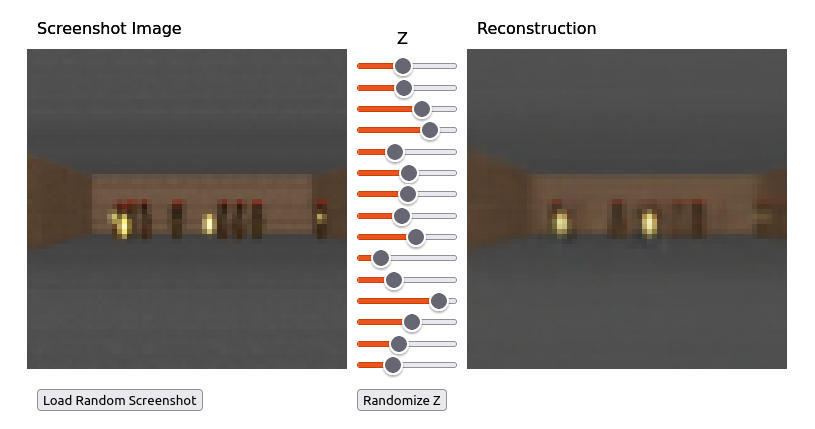
\includegraphics[width = 1.0\textwidth]{imgs/doomviz_latents}
  \caption{Latente Repräsentation von DoomViz aus der Live-Demonstration der World Models \cite{NEURIPS2018_2de5d166}, \cite{worldmodels2023diffdriveimg}}
  \label{img:DoomViz}
\end{figure}

Darauf aufbauend entwickelt Hafner et. al die Dreamer-Architektur als Erweiterung der
World Models und wendet diese erfolgreich auf die MuJoCo Spiele zum Erlernen der
Fortbewegung mit humanoiden Körpern an. Insbesondere ist Dreamer ebenfalls in der Lage,
die Spiele anhand von Videodaten aus der Vogelperspektive zu lernen, was zuvor nur mit
sehr spezialisierten und ressourcenintensiven Lernverfahren möglich war. Namesgebend
für Dreamer ist die Idee, dass während des Träumens anhand von echten Erfahrungen
hypothetische Szenarien halluziniert werden. Wie bei den World Models lernt der Agent
nicht in der echten Simulation, sondern in Träumen, die mit einer kurzen Sequenz aus
echten Situationen starten und dann durch das Dynamikmodell fortgeführt werden,
je nachdem welche Aktionen der Agent auswählt.\\

Unterschiede zwischen den World Models und der Dreamer-Architektur bestehen vor allem
in der latenten Repräsentation und dem zugehörigen VAE, um diese zu extrahieren. Dreamer
verwendet seit Version 2 eine kategorische anstatt einer kontinuierlichen Repräsentation.
Hintergrund hierfür ist, dass die damit verbundene Diskretisierung das Erlernen von
Konzepten erzwingt. Mit 32 Klassifikationen und jeweils 32 Klassen ergeben sich $32^{32}$
mögliche Repräsentationen, was immer noch mehr als ausreichend ist, um vielfältige
Situationen abzubilden. Zudem enthält die latente Repräsentation selbst bereits
Informationen bezüglich der Dynamiken der wahrgenommenen Videosequenz, indem der Zustand
der vom Dynamikmodell verarbeiteten Videosequenz vorheriger Standbilder konkateniert wird.
Dies stellt dem Agent hochwertige Informationen bezüglich der Dynamiken seiner Umgebung
zur Verfügung.\\

Ein weiterer, wichtiger Unterschied besteht in der Art, wie die Modelle trainiert werden.
Im Gegensatz zu den World Models lernt Dreamer nicht zuerst einen VAE, dann ein
Dynamikmodell und trainiert schließlich den Agent. Stattdessen wird bereits während VAE
und Dynamikmodell noch lernen auch der Agent trainiert. Dies ist notwendig, da der Agent
für das Sammeln der Trainingsdaten zur Anpassung des Umgebungsmodells verwendet wird,
um mit der Zeit brauchbare Repräsentationen der Realität und ein gutes Dynamikmodell
zu erhalten. Damit die echte Trainingsumgebung möglichst ganzheitlich exploriert wird,
ist es insbesondere nicht ausreichend, zufällige Aktionen auszuführen, weshalb ein bereits
gut trainierter Agent benötigt wird. Daher trainieren Umgebungsmodell und Agent ähnlich
wie Generator und Discriminator bei GANs immer abwechselnd, um sich mit der Zeit
gegenseitig zu steigern.
